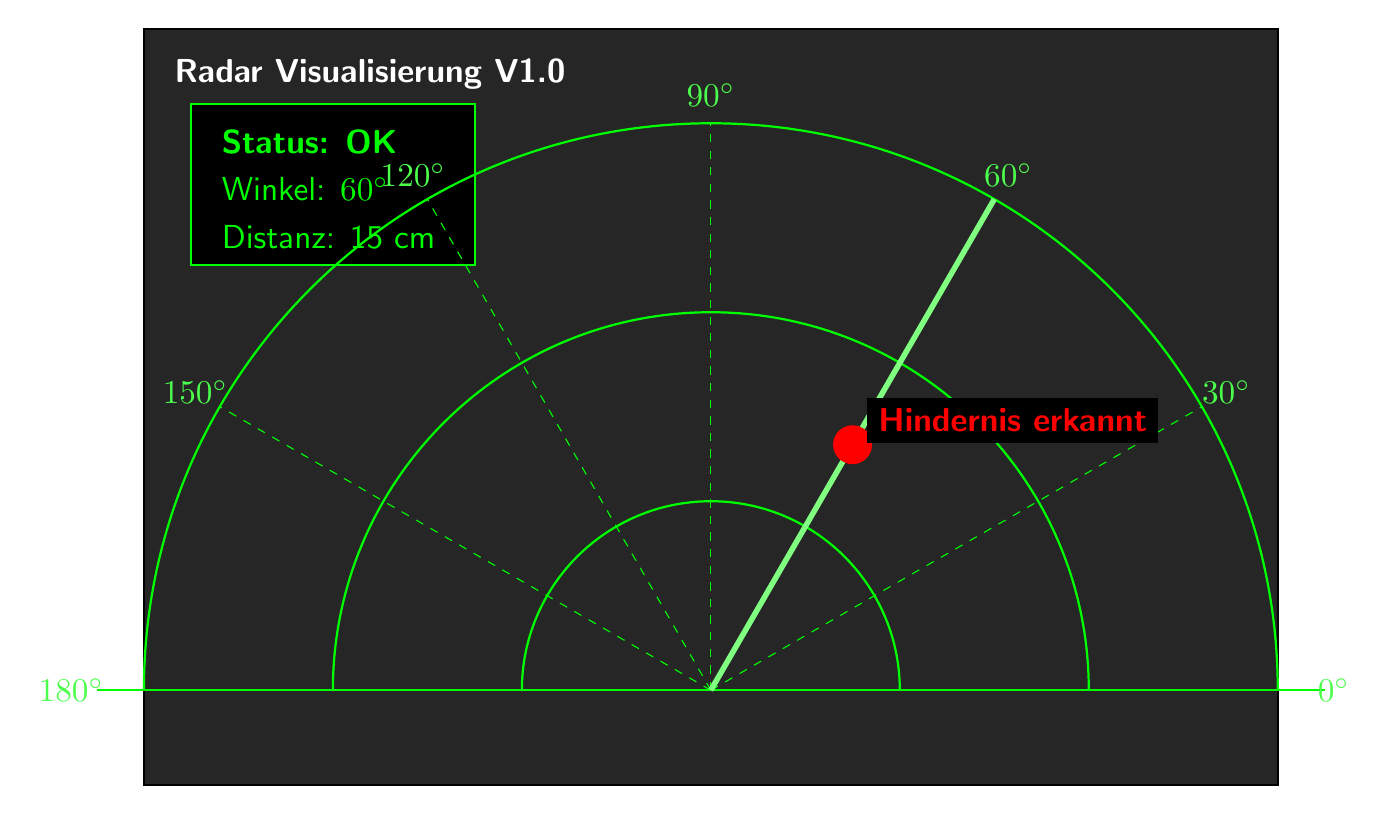
\begin{tikzpicture}[scale=1.2, transform shape, font=\sffamily]
	% Fensterrahmen
	\draw[thick, fill=black!85] (0,0) rectangle (12,8);
	\node[text=white, anchor=north west] at (0.2, 7.8) {\textbf{Radar Visualisierung V1.0}};
	
	% Status Box
	\draw[thick, fill=black, draw=green] (0.5, 5.5) rectangle (3.5, 7.2);
	\node[text=green, anchor=west] at (0.7, 6.8) {\textbf{Status: OK}};
	\node[text=green, anchor=west] at (0.7, 6.3) {Winkel: $60^\circ$};
	\node[text=green, anchor=west] at (0.7, 5.8) {Distanz: 15 cm};
	
	% Radar Gitter (Zentrum bei x=6, y=1)
	\begin{scope}[shift={(6,1)}]
		% Halbkreise (Abstandslinien)
		\foreach \r in {2, 4, 6} {
			\draw[green, thick] (\r,0) arc (0:180:\r);
		}
		% Grundlinie
		\draw[green, thick] (-6.5, 0) -- (6.5, 0);
		
		% Winkellinien
		\foreach \a in {30, 60, 90, 120, 150} {
			\draw[green, dashed] (0,0) -- (\a:6);
			\node[text=green!70, anchor=center] at (\a:6.3) {$\a^\circ$};
		}
		\node[text=green!70, anchor=west] at (6.3, 0) {$0^\circ$};
		\node[text=green!70, anchor=east] at (-6.3, 0) {$180^\circ$};
		
		% Scan-Linie (aktueller Winkel bei 60 Grad)
		\draw[green!50!white, line width=2pt] (0,0) -- (60:6);
		
		% Hindernis (roter Punkt)
		\filldraw[red] (60:3) circle (0.2);
		\node[text=red, right, fill=black] at (60:3.3) {\textbf{Hindernis erkannt}};
	\end{scope}
\end{tikzpicture}